\documentclass[oneside,a4paper,12pt]{book}

\usepackage[spanish]{babel}
\usepackage[utf8]{inputenc}
\usepackage{geometry}
\usepackage{makeidx}
\usepackage{url}
\usepackage{graphicx}
\usepackage{color}
\usepackage{caption}
\usepackage{acronym}
\usepackage{hyphenat}
\usepackage{a4wide}
\usepackage[normalsize]{subfigure}
\usepackage{float}
\usepackage{titlesec}
\usepackage[Lenny]{fncychap}
\usepackage{listings} % para poder hacer uso de "listings" propios (p.ej. códigos)
\usepackage{eurosym} % para poder usar el símbolo del euro con \euro {xx}
\usepackage{hyperref} % TODO: añade la opción hidelinks para imprimirlo (los enlaces no aparecerán resaltados)

% Para que no parta las palabras
\pretolerance=10000

\newcommand{\bigrule}{\titlerule[0.5mm]} \titleformat{\chapter}[display] % cambiamos el formato de los capítulos
{\bfseries\Huge} % por defecto se usaron caracteres de tamaño huge en negrita
{% contenido de la etiqueta 
\titlerule % línea horizontal 
\filright % texto alineado a la derecha 
\Large\chaptertitlename\ % capítulo e índice en tamaño large
\Large % en lugar de 
\Huge \Large\thechapter} 
{0mm} % espacio mínimo entre etiqueta y cuerpo
{\filright} % texto del cuerpo alineado a la derecha
[\vspace{0.5mm} \bigrule] % después del cuerpo, dejar espacio vertical y trazar línea horizontal gruesa
\geometry{a4paper, left=3.5cm, right=2cm, top=3cm, bottom=2cm, headsep=1.5cm}


% Bibliografa
\let\OLDthebibliography=\thebibliography
\def\thebibliography#1{\OLDthebibliography{#1}
  \addcontentsline{toc}{chapter}{\bibname}}


\makeindex

\begin{document}


\thispagestyle{empty}

\begin{titlepage}
	\begin{center}
		\vspace*{3mm}
		\begin{center}
			\includegraphics[width=0.4\linewidth]{imagenes/logo.jpg}
		\end{center}
		\vspace{6.0mm}
		
		\fontsize{15.5}{14}\selectfont ESCUELA TÉCNICA SUPERIOR DE INGENIERÍA DE TELECOMUNICACIÓN
		\vspace{13mm}
		
		\fontsize{14}{14}\selectfont GRADO EN INGENIERÍA DE ROBÓTICA SOFTWARE
		
		\vspace{70pt}
		
		\fontfamily{lmss}\fontsize{15.7}{14}\selectfont \textbf{TRABAJO FIN DE GRADO} 
		
		\vspace{20mm}
		\begin{LARGE}
			Ejercicios Sigue-Persona para la plataforma académica Robotics Academy, usando un robot real y simulado en ROS2
		\end{LARGE}
		
		\vspace{20mm}
		
		\begin{large}
			Autor: Carlos Caminero Abad
			
			Tutor: Dr. Jose María Cañas Plaza
			
			\vspace{10mm}
		\end{large}
		\begin{normalsize}
			Curso académico 2021/2022		
		\end{normalsize}
		\vspace{10mm}
		
	\end{center}
	
\end{titlepage}

\thispagestyle{empty}

\pagenumbering{roman}
\chapter*{Agradecimientos}

El final ha llegado. Escribiendo estas palabras, me acuerdo de todas aquellas personas que han estado presentes a lo largo de mi vida y de este viaje, y que gracias a ellos estoy aquí, a unos días de presentar un proyecto que marcará el final de una de las etapas de mi vida y el principio de otra.\\

Quisiera dar las gracias a mis padres y a mi hermano. Siempre han estado conmigo, apoyándome y ayudándome cuando lo he necesitado. Gracias a mis padres, conocí este grado universitario, y haberlo elegido ha sido una de las mejores decisiones que he tomado en mi vida. Siempre les estaré agradecido.\\

Quisiera agradecer a mis amigos de Yepes por todos los buenos momentos compartidos. Por todas aquellas cenas, en las que nos desahogábamos de nuestros problemas y por todo el apoyo y ánimo que me han transmitido. Es un placer compartir esta vida con gente tan excelente como ellos.\\

Por otra parte, agradezco a mis compañeros de clase por estos cuatro años que, a pesar de compartir duras y difíciles experiencias como la pandemia, también he podido compartir buenos momentos de satisfacción y alegría con ellos.\\ 

Por último, quería agradecer a todos mis profesores por su dedicación e interés por la enseñanza que me han transmitido y en especial, a mi tutor Jose María, por haber estado orientándome a lo largo de todos estos meses dedicados al proyecto. Gracias por toda tu dedicación y animos, y por tu ayuda cuando me encontraba bloqueado por el camino. Ha sido todo un honor haberte tenido como profesor y como tutor.\\

\begin{center}
	¡Muchas gracias a todos!
\end{center}

\chapter*{Resumen}

La Robótica es un sector en constante crecimiento.
Cada vez es más importante el perfil del Ingeniero en Robótica Software para la programación de Robots y Automatismos en esta nueva era digital.
Por ello, es necesario la correcta formación del Ingeniero a través de la accesibilidad
y disponibilidad de los recursos educativos que fomentarán su aprendizaje autodidacta.\\

El objetivo del siguiente Trabajo Fin de Grado (TFG) es desarrollar e implementar 2 nuevos ejercicios educativos para la plataforma
de enseñanza universitaria Unibotics consistentes en programar un robot modelo Turtlebot 2 de Yujin para que sea capaz de seguir a
una persona tanto en un entorno real como en un entorno simulado (un hospital). Con ello, los alumnos y otros usuarios adquirirán las destrezas necesarias 
para la programación de una tarea muy solicitada en la Robótica de Servicio. Aprenderán a seguir a una persona usando un framework de
Redes Neuronales que ayudarán a la detección.\\

La incorporación de estos 2 nuevos ejercicios se aplicarán a una nueva rama de desarrollo para la plataforma Unibotics que usa la distribución ROS Foxy como base.
Además, se habrá logrado la migración y adaptación del modelo simulado del Turtlebot2 de ROS Noetic a ROS Foxy para futuros usos.

\cleardoublepage

\chapter*{Acrónimos\markboth{Acrónimos}{Acrónimos}}

\begin{acronym}
	\acro{CNN}{\emph{Convolutional Neural Network}}
	\acro{CPU}{\emph{Central Processing Unit}}
	\acro{CSS}{\emph{Cascading Style Sheets}}
	\acro{DNN}{\emph{Deep Neural Network}}
	\acro{FSM}{\emph{Finite State Machine}}
	\acro{GPU}{\emph{Graphics Processing Unit}}
	\acro{GUI}{\emph{Graphical User Interface}}
	\acro{HAL}{\emph{Hardware Abstraction Layer}}
	\acro{HTML}{\emph{HiperText Markup Language}}
	\acro{HTTP}{\emph{HiperText Transfer Protocol}}
	\acro{IA}{\emph{Inteligencia Artificial}}
	\acro{LIDAR}{\emph{Laser Imaging Detection and Ranging}}
	\acro{ML}{\emph{Machine Learning}}
	\acro{PID}{\emph{Proportional-Integral-Derivative}}
	\acro{RNA}{\emph{Redes Neuronales Artificiales}}
	\acro{ROS}{\emph{Robot Operating System}}
	\acro{SDK}{\emph{Software Development Kit}}
	\acro{TCP}{\emph{Transmission Control Protocol}}
	\acro{UDP}{\emph{User Datagram Protocol}}
	\acro{URDF}{\emph{Unified Robot Description Format}}
	\acro{USB}{\emph{Universal Serial Bus}}
	\acro{XML}{\emph{eXtensible Markup Language}}
\end{acronym}

\cleardoublepage

\tableofcontents

\listoffigures

\pagestyle{empty}

\cleardoublepage


\mainmatter

\chapter{Introducción}
\label{cap:capitulo1}
\setcounter{page}{1}
\pagestyle{plain}

La tarea Sigue-Personas es una de las más empleadas y solicitadas en los Robots de Servicio para multitud de sectores que incorporan soluciones robóticas. El siguiente TFG propone desarrollar dos nuevos ejercicios para la plataforma Unibotics con el objetivo de que los usuarios programen un robot Turtlebot2 tanto en simulado como en real para que realice dicha tarea.\\

Este primer capítulo trata de presentar el estado actual de varios campos de la Robótica que están directamente relacionados con este proyecto para poner en contexto al lector y facilitar su lectura.\\

Por un lado presentaremos la Robótica Móvil, un sector de la robótica que está en constante crecimiento y muy presente en la Robótica de Servicio; por otra parte, introduciremos las Redes Neuronales, un avance significativo en IA que ha permitido realizar aplicaciones muy robustas basadas en la percepción y el razonamiento; y por último hablaremos de la Robótica Educativa, e introduciremos varias plataformas como TheConstruct, Robotics Academy, o Unibotics siendo estas dos últimas las que incorporarán el ejercicio educativo Sigue-Persona.



\section{Robótica Móvil}
\label{sec:robotica_movil}

La robótica es la ciencia que engloba varias ramas tecnológicas o disciplinas, con el objetivo de diseñar máquinas (``robots'') que sean capaces de realizar tareas automatizadas o de simular el comportamiento humano o animal, en función de la capacidad de su software. \cite{revistaderobots}. Su término se remonta a la obra de ciencia ficción escrita por Isaac Asimov: Yo, Robot. (1950)\\

Una vez que la robótica emerge a partir de mediados del siglo XX, surgen 2 sectores: la Robótica Industrial y la Robótica de Servicio. Los \textbf{Robots industriales} se encargan de realizar tareas automatizadas y muy repetitivas en entornos industriales, donde el entorno es controlado. Los \textbf{Robots de Servicio} son aquellos que realizan tareas útiles para el ser humano proporcionándole un servicio. Destacan los robots móviles que permiten desplazarse de un sitio a otro, sin embargo el entorno en el que se enfrentan es bastante heterogéneo, por tanto su software tiene que ser muy robusto para adaptarse correctamente a los cambios.\\

Un \textbf{robot móvil} un sistema electromecánico capaz de desplazarse de ma­nera autónoma sin estar sujeto físicamente a un solo punto. Posee sensores que permiten monitorear a cada momento su posición relativa a su punto de origen (odometría) y a su punto de destino. Normalmente su control es en lazo cerrado. Se clasifican en robots móviles de \textbf{locomoción con ruedas}, \textbf{locomoción con patas} y \textbf{locomoción con orugas}.  Los primeros son más fáciles de controlar pero no se adaptan bien a muchas superficies, sin embargo los robots con patas (cuadrúpedos o bípedos) se adaptan muy bien a distintas superficies pero requieren varios controladores para mantener su equilibrio tanto estático como dinámico.




\subsection{Evolución Histórica}
\label{subsec:evolucion_historica}

Podemos destacar varios hechos importantes a lo largo del siglo XX y principios del XXI que 
marcaron grandes avances en la robótica:

\begin {itemize}
	\item En 1952 aparece la primera máquina de control numérico del MIT que era capaz de automatizar algunas tareas industriales.
	\item En 1961, la compañía Unimates introdujo el primer robot industral en la General Motors.
	\item En 1966, comenzó el desarrollo del primer robot móvil llamado Shakey [Nilsson, 1984]. \ref{fig:shakey}
	\item En los años 70, NASA desarrolló MARS-ROVER, una plataforma móvil que integraba un brazo mecánico, sensores de proximidad, un dispositivo telemétrico láser y cámaras estéreo
	\item En 1997, la NASA envió a Marte un dispositivo móvil llamado Sojourner Rover, para enviar fotografías a la Tierra del planeta rojo. Además, la empresa HONDA sacó el primer humanoide capaz de imitar comportamientos humanos
	\item En 2000, Honda presenta el robot Asimo.
	\item En 2004, Qrio de Sony, un pequeño robot humanoide capaz de correr, bailar, y reconocer caras.
	\item En 2008, SoftBank Robotics presenta el Robot Nao, un robot bípedo dedicado a interactuar con el ser humano y ser muy amigable
	\item En 2013, Boston Dynamics saca a la luz el robot Atlas, un humanoide con actuadores neumáticos. La empresa lo usa para imitar el comportamiento humano llevándolo a otro nivel haciendo acrobacias o incluso parkour.
	\item En 2014, SoftBank Robotics presenta el robot Pepper, robot con forma humana pero se desplaza con ruedas. Se ha usado sobre todo como robot guía, recepcionista y en exhibiciones, sin embargo, fue abandonado en 2021
	\item En 2020, Boston Dynamics saca a la venta el robot cuadrúpedo que imita el comportamiento de un perro llamado Spot, que se usa en algunas fábricas para transportar materiales o realizar tareas de mantenimiento
\end{itemize}

\begin{figure} [h!]
  \begin{center}
    \includegraphics[width=5cm]{imagenes/shakey.jpg}
  \end{center}
  \caption[Shakey (1966-1972)]{Shakey (1966-1972) \cite{shakey-the-robot}.}
  \label{fig:shakey}
\end{figure}\



\subsection{Aplicaciones actuales}
\label{subsec:aplicaciones_actuales}



\section{Redes Neuronales Artificiales (RNA)}
\label{sec:redes_neuronales}

Según \emph{Arthur Samuel}, el Aprendizaje Automático o Machine Learning es el ``campo de estudio que otorga a los ordenadores la capacidad de aprender sin ser programados explícitamente''. Para ello se emplean diversas técnicas dependiendo del objetivo deseado: Regresión Lineal, Regresión Logística, K-NN, K-Means, SVM, Redes Neuronales, Q-Learning, etc.
\\

Cuando incorporamos una RNA, lo que queremos es que nuestro programa o aplicación sepa \textbf{clasificar} unos datos de entrada con su correspondiente salida, habiendo entrenado previamente un modelo computacional inspirado en el cerebro humano. Para ello se le proporciona un set de datos de entrenamiento, donde indicamos, por cada muestra, a qué clase pertenece (Aprendizaje Supervisado). De esta forma, ajustando los valores de unos pesos que se utilizan en el entrenamiento, conseguiremos un nivel de clasificación determinado.\\

Una aplicación de Redes Neuronales es la detección mediante Vision Artificial de objetos. Para ello, se usan modelos de redes de varias capas con un gran número de neuronas (Deep Learning) y de esta forma conseguimos dada una imagen detectar ciertos objetos solicitados como puede ser fruta, coches, utensilios o incluso hasta personas y animales.\\

Típicamente, una Red Neuronal consta de un conjunto de capas formado por varias neuronas que se encuentran interconectadas. Suelen dividirse en 1 capa de entrada, 1 o más capas ocultas y 1 capa de salida. Pero, ¿cómo funciona una neurona?\\

Una neurona, tal y como se muestra en la figura \ref{fig:neurona} está formada pos los siguientes elementos:
\begin{itemize}
	\item \textbf{Valores de Entrada}: Puede ser tanto los valores de las \textbf{características} de cada muestra como la salida de la neurona de una capa anterior.
	\item \textbf{Pesos}: Son unos valores que se optienen al final de la etapa de entrenamiento.
	\item \textbf{Sumatorio}: Esta formado por los productos de los Valores de Entrada por sus correspondientes Pesos
	\item \textbf{Función de Decisión/Activación}: Es una función matemática que se aplica al sumatorio: Lineal, Escalón, Sigmoide, etc
	\item \textbf{Salida}: Es el valor de la función de decisión. Dependiendo de la función de activación usada, la salida será distinta.
\end{itemize}

\begin{figure} [h!]
  \begin{center}
    \includegraphics[width=15cm]{imagenes/neurona.png}
  \end{center}
  \caption[Modelo computacional de una neurona]{Modelo computacional de una neurona \cite{AIMA}}
  \label{fig:neurona}
\end{figure}


\subsection{Redes Neuronales Convolucionales (CNN)}
\label{subsec:redes_convolucionales}

\subsection{YOLO}
\label{subsec:yolo}

\subsection{SSD}
\label{subsec:SSD}

\section{Educación en Robótica}
\label{sec:educacion_robotica}

\subsection{Grado en Ingeniería de Robótica Software (URJC, España)}
\label{subsec:grado_robotica_software}
La Universidad Rey Juan Carlos (España) imparte en el campus de Fuenlabrada, el grado en Ingeniería de Robótica Software (primer año: 2018) para enseñar a los futuros ingenieros interesados en este campo a programar la \textbf{inteligencia} de los robots del futuro.\\

Tal y como indica el título del grado, se trata de una carrera universitaria de programación, donde los alumnos abarcarán varios temas como por ejmplo Inteligencia Artificial, visión artificial, programación de lenguajes de alto nivel (C++, Python...), Seguridad, Drones, robots de servicio, robótica industrial, y mucho más. Las clases se imparten tanto en salas de ordenadores con sistemas operativos Linux (distribución Ubuntu) como en el laboratorio de Robótica, donde los alumnos podrán programar directamente robots reales.\\

El robot usado en este Trabajo Fin de Grado es un modelo Turtlebot 2 de Yujin. Consta de una base (kobuki) similar a la de un robot de limpieza con sensores de contaco (bumpers), y un soporte encima que le permite incorporar un RPLIDAR, una cámara, y colocar el portátil del estudiante cuando desarrolla una solución al problema.

\subsection{The Construct}
\label{sec:the_construct}
The Construct es una organización que mantiene una plataforma para aprender robótica con ROS, un framework para programar robots. Imparten varios cursos donde los usuarios acceden a máquinas virtuales con un Linux instalado y todas las dependencias adquiridas. 

\subsection{Robotics Academy}
\label{sec:robotics_academy}
Robotics Academy \cite{robotics-academy} es una colección de ejercicios y desafíos para aprender robótica. Está mantenido por la organización JdeRobot. Sus ejercicios abarcan varios temas: drones, robótica móvil, visión artificial, coches autónomos, robótica industrial, etc. Además es una plataforma Open Source, por lo que cualquier interesado/a puede contribuir desde Github.\\

En sus orígenes, solo se podía ejecutar sobre un sistema operativo Linux, pero desde sus últimas versiones puede ejecutar también sobre Windows y MAC, gracias a la incorporación de plantillas web que se ejecutan en un navegador estableciendo una conexión a través de WebSockets con un contenedor docker que lanza el usuario, permitiendo de esta manera, el despliegue de los ejercicios sobre un sistema operativo virtualizado y con todas sus dependencias ya instaladas.\\

Los usuarios una vez que escogen un ejercicio, lanzan un contenedor docker indicado y automáticamente tienen acceso a una dirección web local donde pueden empezar a programar. La plantilla web incorpora un Editor de Texto y la posibilidad de visualizar un entorno de Gazebo y un terminal mediante una conexión VNC con el contenedor. En la figura \ref{fig:rob-ac-web-template} vemos un ejemplo de plantilla web correspondiente al ejercicio \textit{Follow Person}. La programación se realiza con Python (un lenguaje fácil de entender y aprender, y muy usado en la Robótica).\\

\begin{figure} [h!]
  \begin{center}
    \includegraphics[width=15cm]{imagenes/robotics-academy-web-template.png}
  \end{center}
  \caption[Robotics Academy (Web Template)]{Robotics Academy (Web Template)}
  \label{fig:rob-ac-web-template}
\end{figure}

Una ventaja de usar Robotics Academy, es que permite al usario centrarse única y exclusivamente con el algoritmo que tenga que implementar. Toda la complejidad relacionada con la comunicación con el hardware del robot: motores, laser, cámara, etc. que, por lo general se realiza mediante ROS (un framework para programar Robots) queda encapsulado por 2 módulos: HAL y GUI. De esta manera, el usuario dispone de una API de HAL (Hardware Abstración Layer) para comandar a los actuadores o recibir información de los sensores, y una API de GUI (Graphical User Interface) para visualizar por el navegador información como puede ser una imagen, un mapa o incluso vectores.\\

\subsection{Unibotics}
\label{sec:unibotics}

\textbf{Unibotics} es una plataforma de Robótica que incorpora parte de la coleción de ejercicios de Robotics Academy. Con Unibotics, JdeRobot da un nuevo paso, permitiendo a los usuarios registrarse en un servidor donde pueden guardar sus códigos, acceder cuando deseen, y además, poder contar con la posibilidad de lanzar los ejercicios en un servidor remoto de manera que los usuarios no necesiten instalar docker en sus sistemas operativos.\\

Una vez que el usuario introduce sus credenciales y accede a su sesión, tiene una lista de ejercicios disponibles [Figura \ref{fig:menu-unibotics}], que funcionan de la misma manera que aquellos que proporciona \textit{Robotics Academy}. Actualmente todos los ejercicios disponibles están implementados usando dentro del sistema operativo virtual la distribución ROS Noetic como báse.

Con los 2 nuevos ejercicios Sigue-Personas que explicaremos en este proyecto, pretendemos integrarlos en Unibotics usando ROS Foxy como base. De esta manera, marcaremos un inicio para la migración de varios ejercicios de ROS Noetic a ROS Foxy

\begin{figure} [H]
  \begin{center}
    \includegraphics[width=15cm]{imagenes/unibotics-menu.png}
  \end{center}
  \caption[Unibotics (Menú)]{Unibotics (Menú)}
  \label{fig:menu-unibotics}
\end{figure}






\chapter{Objetivos}
\label{cap:capitulo2}

Capitulo 2

\section{Sección 1}
\label{sec:miseccion}

\chapter{Herramientas utilizadas}
\label{cap:capitulo3}

El desarrollo de los 2 nuevos ejercicios de Robotics Academy han abarcado varios campos: programación, Docker, modelado y simulación de robots, ROS y ROS2, visión artificial, machine learning, desarrollo web... por lo que es necesario introducir y describir las herramientas y tecnologías utilizadas.




% -- SECCIÓN C++
% ----------------
\section{C++}
\label{sec:c++}

C++ es un lenguaje de programación diseñado en 1979 por Bjarne Stroustrup. Deriva del lenguaje C, y destaca principalmente porque incorpora el paradigma de la Programación Orientada a Objetos (POO). Además, incorpora una gran cantidad de nuevas librerías para facilitar la programación como por ejemplo las librerías estandar y STL (Standard Template Library).\\

\begin{code}[H]
\begin{lstlisting}[language=C++]
#include <iostream>

int main(int argc, char ** argv)
{
	std::cout << "Hello World!\n";
	return 0;
}
\end{lstlisting}
\caption[Hola mundo en C++]{Hola mundo en C++}
\label{cod:holamundo_cplusplus}
\end{code}

\textbf{¿Cuál ha sido la utilidad de C++ en este proyecto?} La programación de un \textbf{plugin} \footnote{\textbf{Plugin}: Complemento que añade una funcionalidad extra o mejora a un programa} que permite mover a una persona simulada en Gazebo \footnote{\textbf{Gazebo}: simulador robótico} con el teclado.\\




% -- SECCIÓN PYTHON
% -------------------
\section{Python}
\label{sec:python}

Python es un lenguaje de programación interpretado \footnote{\textbf{Interprete} (programación): programa informático que se encarga de ejecutar las instrucciones de otro programa sin compilación previa} que destaca por su legibilidad, facilidad y soportabilidad a la programación Orientada a Objetos. Posee características particulares que lo diferencian de otros lenguajes de programación como puede ser el uso estricto de indentación en bloques de código.\\

\begin{code}[H]
\begin{lstlisting}[language=Python]
print("Hola mundo")
\end{lstlisting}
\caption[Hola mundo en Python]{Hola mundo en Python}
\label{cod:holamundo_python}
\end{code}

\textbf{¿Cuál ha sido la utilidad de Python en este proyecto?} El desarrollo de la infraestructura interna que da soporte a los dos nuevos ejercicios de Robotics Academy, programación de nodos de ROS (más en la sección \ref{sec:ros}) y ficheros de lanzamiento, creación de los módulos HAL y GUI y desarollo de la solución a los ejercicios.




% -- SECCION ROS
% ----------------
\section{ROS (Robot Operating System)}
\label{sec:ros}
ROS (Robot Operating System) es un middleware \footnote{\textbf{Middleware}: software que se sitúa entre las aplicaciones y el sistema operativo} que ayuda a la programación de robots a través de varias librerías y herramientas desarrolladas por la comunidad de software libre. Entre las ayudas que proporciona este framework están la abstracción del hardware, controladores de dispositivos, herramientas de visualización y geometría espacial entre otros.\\

Desde un principio, ROS se ha ejecutado sobre sistemas operativos de tipo Unix (Ubuntu - principal), aunque han ido surgiendo versiones beta para otros sistemas como Windows o MacOS X. La primera distribución de ROS salió en 2010 (ROS Box Turtle) y a partir de ahí han ido surgiendo nuevas distribuciones siendo la actual y estable ROS Noetic.\\

El funcionamiento de ROS se basa en una arquitectura cliente-servidor centralizado donde un nodo principal se encarga del intercambio de mensajes entre otros nodos que forman la aplicación (remotos o locales), los cuales se comportan como publicadores o suscriptores del proceso de comunicación. El objetivo es dividir el software robótico en secciones o nodos que se encargan de realizar tareas específicas de manera paralela: recogida de datos de la cámara, ejecución de una máquina de estados o árboles de comportamiento (Behavior Trees), recogida de las lecturas del láser, navegación, etc.\\

El intercambio de mensajes se realiza a través \textbf{topics}. Un nodo puede tener \textbf{publicadores}, \textbf{suscriptores} o ambos. Cuando un nodo publica un mensaje lo hace a través de un topic que gestiona el nodo maestro. Si otro nodo quiere leer ese mensaje tendrá que suscribirse al tópic correspondiente. Por ejemplo: en nuestro robot Turtlebot2 podemos comandar velocidades enviando mensajes de tipo \textbf{geometry\_msgs.msg.Twist} a través del topic \textbf{/cmd\_vel}. En la figura se puede ver con más detalle \ref{fig:ros_master_comunicacion}\\

\begin{figure} [H]
  \begin{center}
    \includegraphics[width=15cm]{imagenes/ros_master_communication.png}
  \end{center}
  \caption{Comunicación del nodo Master con los nodos Intermedios (ROS)}
  \label{fig:ros_master_comunicación}
\end{figure}\

ROS incorpora un conjunto de librerías para ser usadas en C++ y Python. Con estos lenguajes de programación podemos desarrollar los nodos de los paquetes que tendrá nuestra aplicación. También incorpora un conjunto de comandos de \textbf{Shell} (términal) para hacer tareas de depuración, creación, compilación, etc.\\

En 2016 surge ROS 2, nuevo framework basado en ROS con muchas más mejoras como la \textbf{calidad de servicio}, los \textbf{lifecycle nodes} o \textbf{seguridad} (DDS) para asegurar la autenticación de los nodos y la integridad de los mensajes. Al igual que con ROS 1 ha tenido varias distribuciones siendo la primera \textbf{ROS Ardent}. La versión más reciente y estable es \textbf{ROS Foxy}, que es la que hemos usado en este proyecto.\\

Aprender ROS no es una tarea sencilla y requiere mucha dedicación y esfuerzo. Por lo tanto, el objetivo de Robotics Academy es proporcionar una interfaz de programación sencilla para programar robots sin necesidad de saber ROS. Es decir, el usuario tiene acceso a unas librerías HAL y GUI, las cuales usan por debajo nodos de ROS.\\

\textbf{¿Cuál ha sido la utilidad de ROS2 en este proyecto?} Crear los ficheros \textbf{interfaces} (laser.py, motors.py, camera.py, ...) que se comunican con los topics necesarios para el control del robot Turtlebot 2.




% -- SECCION URDF
% -----------------
\section{URDF}
\label{sec:urdf}

\textbf{URDF (United Robotics Description Format)} es un lenguaje de marcado para describir robots (eslabones, uniones, jerarquías, modelo visual, modelo de collisión, modelo inercial, controladores, etc) que usa la gramática de XML. Se utiliza tanto para robots reales como simulados.\\

Por lo general el robot se divide en su mayoría en eslabones (links) y uniones entre eslabones (joints), de manera que se forma un árbol jerárquico desde un eslabón principal (root) hasta los eslabones terminales.\\

Para definir un link hay que proporcionar un modelo visual, un modelo de colisión y un modelo inercial. Después se define el joint que une el eslabón que hemos definido con otro mediante una jerarquía de padres e hijos. En el siguiente código podemos ver un ejemplo de como se definiría un cubo de 1 metro por lado para su representación en un simulador.\\

\begin{code}[H]
\begin{lstlisting}
<?xml version="1.0"?>
<robot name="simple_cube">
	<link name="base_link">
		<visual>
			<origin xyz="0 0 0"/>
			<geometry>
				<box size="1.0 1.0 1.0"/>
			</geometry>
		</visual>
		<collision>
			<origin xyz="0 0 0"/>
			<geometry>
				<box size="1.0 1.0 1.0"/>
			</geometry>
		</collosion>
		<inertial>
			<origin xyz="0 0 0" /> 
			<mass value="1.0" />
			<inertia  ixx="1.0" ixy="0.0"  ixz="0.0"  iyy="1.0"  iyz="0.0"  izz="1.0"/>
		</inertial>
	</link>
</robot>
\end{lstlisting}
\caption[Ejemplo de código URDF: Definición de un cubo]{Ejemplo de código URDF: Definición de un cubo}
\label{cod:codigo_urdf}
\end{code}

\textbf{¿Cuál ha sido la utilidad de URDF en este proyecto?} Para la creación del modelo Turtlebot 2 simulado en ROS Foxy.
\begin{figure} [H]
  \begin{center}
    \includegraphics[width=10cm]{imagenes/turtlebot2-sim.png}
  \end{center}
  \caption{Modelo Turtlebot2 simulado (definido mediante URDF)}
  \label{fig:ros_master_comunicación}
\end{figure}\




% -- SECCION XACRO
% ------------------
\section{XACRO}
\label{sec:xacro}

XACRO (XML Macros) es un lenguaje XML diseñado para crear macros \footnote{\textbf{macro}: plantilla que define un patrón} en URDF. Con XACRO conseguimos diseños URDF mucho más legibles y sencillos. De esta manera podemos estructurar el diseño de un robot en componentes más pequeños y repetitivos. Por ejemplo: para el diseño del robot Turtlebot2 creamos una macro que se pueda aplicar a todos las barras verticales que sujetan la estructura del robot.\\

Una vez que tenemos nuestro diseño en XACRO, podemos exportarlo a URDF mediante el paquete de ROS denominado \textbf{xacro}. Su comportamiento es semejante al preprocesador de los lengauejes de programación como C: la macro la sustituye por el código URDF deseado teniendo en cuenta el valor de la variables que haya definido el programador.\\

\textbf{¿Cuál ha sido la utilidad de XACRO en este proyecto?} Diseñar un diseño sencillo y flexible del robot Turtlebot2. En el capítulo \ref{cap:capitulo4} describiremos mejor los detalles mediante algunas muestras del diseño.\\



% -- SECCION HTML Y CSS
% -----------------------
\section{HTML y CSS}
\label{sec:html_css}

\textbf{HTML (HiperText Markup Language)} es un lenguaje de marcado de tipo XML para el diseño de la estructura de las páginas web. Es un lenguaje que entiende el navegador web y se suele acompañar mediante una hoja de estilos que nos proporciona el lenguaje \textbf{CSS (Cascading Style Sheets)} para crear el estilo gráfico de la página web.\\


\begin{code}[H]
\begin{lstlisting}
<p>Esto es un parrafo en HTML</p>
\end{lstlisting}
\begin{lstlisting}
p {
	background-color: #FF0000;
}
\end{lstlisting}
\caption[Ejemplo de HTML y CSS]{Ejemplo de HTML y CSS: Todos los párrafos tienen el fondo rojo}
\label{cod:codigo_urdf}
\end{code}

\textbf{¿Cuál ha sido la utilidad de HTML y CSS en este proyecto?} Diseñar y dar estilo a la plantilla web de los 2 nuevos ejercicios de Robotics Academy. El diseño se base en seguir las plantillas de los demás ejercicios con algunos pequeños cambios e incorporaciones específicos.



% -- SECCION JAVASCRIPT
% -----------------------
\section{Javascript}
\label{sec:javascript}

Javascript es un lenguaje de programación interpretado que destaca por ser utilizado en el lado del cliente, en el Frontend de una página web que lee el navegador. Con Javascript podemos crear páginas web dinámicas a través de la definición de eventos que provocan resultados en el Backend (si tiene) o en la propia estructura HTML. Javascript puede usarse para multitud de tareas: Websockets, juegos, animaciones, etc.\\

\textbf{¿Cuál ha sido la utilidad de Javascript en este proyecto?}
En las plantillas web de Robotics Academy se usa Javascript para comunicar los eventos de la página con el fichero maestro de cada ejercicio que se llama \textbf{exercise.py}.\\



% -- SECCIÓN DOCKER
% -------------------
\section{Docker}
\label{sec:docker}

Docker (TODO)


% -- SECCIÓN DESCRIPCION INFRAESTRUCTURA
% ----------------------------------------

\section{Infraestructura Robotics Academy}
\label{sec:infraestructura_robotics_academy}
Una vez que hemos resumido las herramientas usadas podemos recopilarlas y mostrar un esquema génerico de la infraestructura de Robotics Academy:

\begin{figure} [H]
  \begin{center}
    \includegraphics[width=15cm]{imagenes/esquema-robotics-academy.png}
  \end{center}
  \caption{Infraestructura Robotics Academy}
  \label{fig:infraestructura_robotics_academy}
\end{figure}\


\chapter{Soporte de Turtlebot 2 en ROS Foxy}
\label{cap:capitulo4}

% -- INTRODUCCION
% -----------------
En este capítulo se presenta el proceso de \textbf{migración} del robot Turtlebot 2 de ROS Noetic a \textbf{ROS Foxy}. Se describirán todos los cambios relevantes realizados como puede ser la modificación de sus ficheros URDF/XACRO, su lanzamiento en Gazebo a través de los launchers de ROS2 o incluso su integración sobre una imagen Docker.\\

El soporte más estable del Turtlebot 2 se encuentra en la rama de \textbf{ROS Melodic} (tanto real como simulado) aunque también funciona en ROS Noetic \footnote{\textbf{Turtlebot 2 (Noetic)}: \url{https://bitbucket.org/theconstructcore/turtlebot/src/noetic/}}. Sin embargo, para ROS 2 Foxy solamente hay un repositorio \footnote{\textbf{Base Kobuki (foxy)}: \url{https://github.com/kobuki-base/kobuki_ros}} con los drivers para mover la base kobuki [\ref{sec:kobuki_base}] real (sin  ficheros de lanzamiento para Gazebo).\\

De modo que el \textbf{primer paso} del TFG era dar soporte completo al Turtlebot 2 en ROS Foxy para poder desarrollar los nuevos ejercicios de Robotics Academy. A continuación mostraré en orden los pasos realizados hasta su resultado final.\\


% -- SECCION KOBUKI BASE
% ------------------------
\section{Kobuki Base}
\label{sec:kobuki_base}

El respositorio oficial de kobuki base contiene los siguientes paquetes relevantes:

\begin{itemize}
	\item \textbf{kobuki\_description}: Es el paquete que contiene los ficheros de descripción xacro [\ref{sec:xacro}] y URDF [\ref{sec:urdf}] de la base. Con este directorio se describe el \textbf{árbol de tranformadas} que existen entre todos los links del robot, y de esta manera poder conocer la localización de todos los frames. También se añaden plugins para facilitar el control de movimiento del robot (controladores de velocidad, odometría ...).
	\item \textbf{kobuki node}: Es el paquete que contiene un fichero de configuración denominado \textbf{kobuki\_node\_params.yaml} con el que podemos conectarnos al robot real usando el puerto \textbf{/dev/ttyUSB0}, así como la definición de algunos frames (base, odom). También contiene los ficheros de los nodos necesarios para controlar la base kobuki y su odometría. Oculta al programador la complejidad de comunicarnos directamente con el hardware (motores, leds...) del robot usando nodos ros con publicadores y suscriptores. El nodo que lanza \textbf{kobuki\_ros\_node} se suscribe al tópic \textbf{/commands/velocity} para recibir mensajes de tipo \textbf{geometry\_msgs.msg.Twist} y poder mover mediante velocidad lineal y angular la base del robot. Este directorio no tiene relación con kobuki\_description.
	\item \textbf{kobuki\_keyop}: Es un paquete que nos permite mover la base del robot con el teclado del ordenador. Se crea un nodo que publica por cada pulsación del teclado, un mensaje \textbf{geometry\_msgs.msg.Tiwst} en el topic \textbf{/cmd\_vel} (tendremos que cambiar a \textit{/commands/velocity} si queremos controlar el robot real. Este paquete nos puede ayudar en un principio a comprobar que tenemos conexión con el hardware real.
\end{itemize}

Con estos 3 paquetes tenemos lo necesario para controlar la base del robot. Sin embargo, solo nos sirve para el robot real, y no en simulado. Como se ha mencionado antes, el paquete \textbf{kobuki\_description} no tiene relación con kobuki\_node, solo nos permite visualizar un árbol de transformadas con el visualizador \textbf{RVIZ 2} de modo que el siguiente paso fue representar la base kobuki, mediante los ficheros de descripción, en un escenario de Gazebo.\\




% -- SECCION LANZAMIENTO EN GAZEBO
% ----------------------------------
\subsection{Lanzamiento en Gazebo}
\label{subsec:kobuki_gazebo}

Para conseguir la representación de la base kobuki en Gazebo hice un \textbf{fork}\footnote{\textbf{Kobuki ROS (fork)}: \url{https://github.com/Carlosalpha1/kobuki_ros}} del repositorio oficial e implemente un nuevo paquete llamado \textbf{kobuki\_gazebo}. Dentro incluí ficheros \textbf{launch.py} para lanzar tanto el simulador Gazebo como la base kobuki simulada. A continuación describiremos los ficheros más importantes del nuevo paqueté implementado:

\begin{itemize}
	\item \textbf{empty\_world.launch.py}: Un punto de partida en muchas ocasiones cuando creamos un robot simulado es diseñar un fichero de lanzamiento que únicamente lance un mundo vacío en Gazebo. De esta manera, puedes incluir ese fichero en otros ficheros de lanzamiento y dividimos un problema complejo en varios subproblemas. Para lanzar \textbf{Gazebo} en ROS 2 ejecutamos 2 ficheros de lanzamientos en este orden:
	\begin{enumerate}
		\item \textbf{gazebo\_ros - gzserver.launch.py}: Lanza un servidor gazebo sin ventana, de modo que podemos ejecutar programas sin necesidad de visualizar el resultado en Gazebo.
		\item \textbf{gazebo\_ros - gzclient.launch.py}: Lanza un cliente gazebo que activa una ventana donde podemos ver el mundo solicitado.
	\end{enumerate}
	
	\cleardoublepage
\begin{code}[H]
\begin{lstlisting}[frame=single]
def generate_launch_description():

	ld = LaunchDescription()

	pkg_gazebo_ros = get_package_share_directory('gazebo_ros')
		
	gazebo_server = IncludeLaunchDescription(
		PythonLaunchDescriptionSource(os.path.join(pkg_gazebo_ros, 'launch', 'gzserver.launch.py'))
	)
		
	gazebo_client = IncludeLaunchDescription(
		PythonLaunchDescriptionSource(os.path.join(pkg_gazebo_ros, 'launch', 'gzclient.launch.py'))
	)
	
	ld.add_action(gazebo_server)
	ld.add_action(gazebo_client)
	
	return ld
\end{lstlisting}
\caption[kobuki\_gazebo: empty\_world.launch.py]{kobuki\_gazebo: empty\_world.launch.py}
\label{cod:kobuki_gazebo_empty_world}
\end{code}

	\item \textbf{spawn\_model.launch.py}: Este fichero pasa los datos de descripción \textbf{urdf} de la base kobuki a un parámetro denominado \textbf{/robot\_description}, publica el estado del robot, sus transformadas y ejecuta el fichero de gazebo\_ros \textbf{spawn\_entity.py} para visualizar el modelo en el simulador:
	
\begin{code}[H]
\begin{lstlisting}[frame=single]
kobuki_model = Node(
	package='robot_state_publisher',
	executable='robot_state_publisher',
	parameters=[{'robot_description': robot_desc}],
	arguments=[urdf_file]
)

joint_state_publisher_node = Node(
	package='joint_state_publisher',
	executable='joint_state_publisher',
	name='joint_state_publisher'
)

spawn_entity = ExecuteProcess(
	cmd=['ros2', 'run', 'gazebo_ros', 'spawn_entity.py', '-topic', '/robot_description', '-entity', 'kobuki'], output='screen')
\end{lstlisting}
\caption[kobuki\_gazebo: spawn\_model.launch.py]{kobuki\_gazebo: spawn\_model.launch.py}
\label{cod:kobuki_gazebo_spawn_model}
\end{code}
\end{itemize}

Podremos visualizar la base kobuki en simulado ejecutando los siguientes comandos:\\
\begin{lstlisting}
ros2 launch kobuki_gazebo empty_world.launch.py &
ros2 launch kobuki_gazebo spawn_model.launch.py
\end{lstlisting}\

En la figura \ref{fig:sim_kobuki_base} podréis ver el resultado de la base kobuki simulada en Gazebo
\begin{figure} [H]
  \begin{center}
    \includegraphics[width=10cm]{imagenes/sim_kobuki_base.png}
  \end{center}
  \caption[\textbf{Modelo simulado} de Kobuki Base (ROS 2 Foxy)]{\textbf{Modelo simulado} de Kobuki Base (ROS 2 Foxy)}
  \label{fig:sim_kobuki_base}
\end{figure}\




% -- SECCION IMAGEN DOCKER
% --------------------------
\subsection{Imagen Docker}
\label{sec:kobuki_base_docker}

Para empezar a controlar la base kobuki con un contenedor docker, definimos un fichero Dockerfile con todas las dependencias necesarias junto con los comandos necesarios para lanzar los nodos.\\

En esta dirección, podréis descargar una versión de prueba para mover un robot real Turtlebot 2 en ROS Foxy con el paquete \textbf{kobuki\_keyop} sin necesidad de instalar ROS 2 ni ningún otro paquete: \url{https://hub.docker.com/r/carlosalpha1/kobuki_keyop}. Al lanzar el contenedor mostrará una ventana emergente de un terminal \textbf{xterm} para pulsar las teclas correspondientes que moverán la base del robot.\\

\textbf{Comandos para lanzar el contenedor kobuki\_base}:\\
\begin{lstlisting}
xhost +
docker run -it --rm --device /dev/ttyUSB0 -e DISPLAY=$DISPLAY -v /tmp/.X11-unix:/tmp/.X11-unix carlosalpha1/kobuki_keyop:ros-foxy
xhost -
\end{lstlisting}\

Controlar la base kobuki supone un avance muy significativo para poder usar el robot Turtlebot 2. Solamente haría falta usar paquetes de ROS para el láser y la cámara (tal y como veremos en el capítulo [\ref{cap:capitulo6}]). Sin embargo, aún no tenemos disponible la simulación del robot Turtlebot 2 completo, por lo que en los siguientes apartados integraremos la estructura que soporta la base.\\



% -- SOPORTE TURTLEBOT 2
% ------------------------
\section{Soporte Turtlebot 2}
\label{sec:soporte_turtlebot2}

A parte de la base Kobuki, la otra mitad que caracteriza al Turtlebot 2 es la \textbf{base superior} que permite colocar portátiles, sensores o actuadores. En esta sección abordaremos la migración a ROS Foxy de esta última parte del robot.\\

La \textbf{pregunta}, es \textit{¿por qué no usamos ficheros turtlebot\_description de la rama Noetic o Melodic si el lenguaje URDF es el mismo?} En realidad, el paso de ROS 1 a ROS 2 conlleva cambios tanto en la manera de crear nodos, ficheros de lanzamiento y su funcionamiento interno como en el uso de URDF. El modelo Turtlebot 2, al tener una gran cantidad de ficheros URDF que dependían unos de otros, y estos a su vez de otros paquetes con dependencias de ROS 1, no facilitaba la tarea de obtener un modelo creando únicamente ficheros launch.py como hicimos con la base kobuki.\\

Entonces, la \textbf{solución} fue crear la estructura restante del robot a mano, usando la sintáxis URDF y XACRO, creando un modelo lo más semejante posible al real. A continuación mostraré las fases del desarrollo. Una vez terminado el modelo Turtlebot 2 simulado, tendremos por un lado un directorio con todos los paquetes de kobuki\_base y otro directorio con la definición del nuevo soporte creado.\\



% -- FICHEROS DE CONFIGURACION XACRO
% ------------------------------------
\subsection{Ficheros de Configuración XACRO}
\label{sec:turtlebot2_xacro}

El primer paso de esta segunda parte fue crear el modelo URDF. Usando XACRO me permitió crear \textbf{macros} que facilitara la estructura y la legibilidad del modelo. Con XACRO era sencillo incluir nuevos elementos en el modelo y establecer la jerarquía de transformadas entre links de padres a hijos (siempre es importante indicar las relaciones jerárquicas para poder realizar futuras operaciones basadas en frames).\\

La estructura del nuevo directorio es la siguiente:
\begin{figure}[H]
	\begin{center}
	    \setlength{\fboxsep}{0.5cm}
	    \fbox{
        \begin{minipage}{10cm}
          \dirtree{%
          .1 turtlebot2.
          .2 kobuki\_base.
          .3 kobuki\_ros\_interfaces.
          .3 kobuki\_ros.
          .4 Ficheros de kobuki\_gazebo \ref{sec:kobuki_gazebo}.
          .4 \vdots.
          .2 turtlebot2.
          .3 launch.
          .4 empty\_world.launch.py.
          .4 spawn\_model.launch.py.
          .3 rviz.
          .3 urdf.
          .4 structures.urdf.xacro.
          .4 colors.urdf.xacro.
          .4 turtlebot2.urdf.xacro.
          .4 sensors.
          .5 camera.urdf.xacro.
          .5 lidar.urdf.xacro.
          .3 spawn.sh.
          .3 CMakeLists.txt.
          .3 package.xml.
          }
        \end{minipage}
        }
	    \caption{Estructura de directorios completa del Turtlebot 2 (ROS 2 Foxy)}
	    \label{fig:directorios_turtlebot2}
	\end{center}
\end{figure}\

En el fichero \textbf{colors.urdf.xacro} definimos algunas macros para establecer colores en el modelo de gazebo:\\
\begin{code}[H]
\begin{lstlisting}
<xacro:macro name="create_color" params="name value">
	<material name="${name}">
		<color rgba="${value}"/>
	</material>
</xacro:macro>

<xacro:macro name="gazebo_color" params="link color">
	<gazebo reference="${link}">
		<material>Gazebo/${color}</material>
	</gazebo>
</xacro:macro>

<xacro:create_color name="Gray" value="0.5 0.5 0.5 1"/>
<xacro:gazebo_color link="base_tick1_link" color="Gray"/>
\end{lstlisting}
\caption{Creación y establecimiento de un color a un \textbf{link}}
\label{fig:creacion_color_link}
\end{code}\

En el fichero \textbf{structures.urdf.xacro} definimos 2 macros para crear los links que necesitamos y definimos las \textbf{relaciones jerárquicas} de padres a hijos. Las nuevas macros son \textbf{cylinder\_structure} y \textbf{cube\_structure}, para crear en el fichero turtlebot2.urdf.xacro elementos como los siguientes:
\begin{code}[H]
\begin{lstlisting}
<xacro:cylinder_structure name="base_tick5" x="0.15" y="0.0" z="0.14" length="0.15" radius="0.005" parent="base_link"/>
<xacro:cube_structure name="camera_support_base" x="0.13" y="0" z="0.0975" x_size="0.0175" y_size="0.15" z_size="0.005" parent="middle_base_link"/>
\end{lstlisting}
\caption{Creación de 2 links usando 2 nuevas macros definidas}
\label{fig:creacion_link_macro}
\end{code}\

En el fichero turtlebot2.urdf.xacro incluimos con la macro \textbf{xacro:include} las definiciones URDF de los ficheros del paquete \textbf{kobuki\_description}. Por último, creamos dos ficheros XACRO para colocar una cámara RGBD y un láser 360 grados. Los ficheros de los sensores los podéis ver en este \textbf{enlace}. \footnote{\textbf{Sensores Turtlebot2}: \url{https://github.com/RoboticsLabURJC/2021-tfg-carlos-caminero/tree/main/turtlebot2/turtlebot2/urdf/sensors/}}\\

Mediante este comando podemos generar un fichero urdf con toda la descripción del modelo a partir de turtlebot2.urdf.xacro:\\
\begin{lstlisting}
ros2 run xacro xacro urdf/turtlebot2.urdf.xacro > urdf/turtlebot2.urdf
\end{lstlisting}\




% -- TURTLEBOT 2: LANZAMIENTO EN GAZEBO
% ---------------------------------------
\subsection{Lanzamiento en Gazebo}
\label{sec:turtlebot2_gazebo}

Para la \textbf{visualización} del modelo URDF en Gazebo me basé en los mismos ficheros que hice con la base Kobuki: \textbf{empty\_world.launch.py} y \textbf{spawn\_model.launch.py} [\ref{sec:kobuki_gazebo}]\\

La única diferencia fue definir 3 argumentos por defecto para establecer la \textbf{posición inicial} del robot, para que cuando se quiera importar el modelo en cualquier otro mundo de Gazebo, el programador pueda especificar el punto de inicio. Estos 3 argumentos se pasan al nodo \textbf{spawn\_entity}. A continuación podemos ver la sección referente a la posición inicial del fichero \textbf{spawn\_model.launch.py}:\\
\begin{lstlisting}
	# Set (x, y, z) default position of turtlebot2
	x_pos = LaunchConfiguration('-x', default='0')
	y_pos = LaunchConfiguration('-y', default='0')
	z_pos = LaunchConfiguration('-z', default='0')
	
	spawn_entity_node = Node(
		package='gazebo_ros',
		executable='spawn_entity.py',
		name='entity_spawner',
		output='screen',
		arguments=["-topic", "/robot_description", "-entity", "turtlebot2", "-x", x_pos, "-y", y_pos, "-z", z_pos]
	)
\end{lstlisting}\

Una vez abierto Gazebo, para lanzar el modelo ejecutamos el siguiente comando:\\
\begin{lstlisting}
ros2 launch turtlebot2 spawn_model.launch.py
\end{lstlisting}\

En la figura \ref{fig:evolucion_turtlebot2_sim} podemos ver la evolución del proceso creativo del Turtlebot 2 simulado:
\begin{figure} [H]
  \begin{center}
    \includegraphics[width=10cm]{imagenes/creacion-turtlebot2-sim.png}
  \end{center}
  \caption[Evolución Turtlebot 2 simulado]{Evolución Turtlebot 2 simulado}
  \label{fig:evolucion_turtlebot2_sim}
\end{figure}\


\textbf{Consideraciones a tener en cuenta}: Tanto el modelo Kobuki como el Turtlebot 2 simulado usan un plugin para controlar los motores denominado \textbf{differential\_drive\_controller.so}. Este plugin se suscribe a un topic para controlar la velocidad de las ruedas del robot llamado \textbf{/cmd\_vel} (estándar en ROS), por lo que no coincide con el topic del robot real \textbf{/commands/velocity}.




\chapter{Ejercicios Sigue-Persona en Robotics Academy}
\label{cap:capitulo5}

En este capítulo profundizamos en el proceso creativo de la infraestructura de los dos ejercicios Sigue-Persona para Robotics Academy. Cada uno de ellos tiene dos partes: a) una plantilla Python en la que se ejecuta el ćodigo fuente del usuario (\texttt{exercise.py}) y b) una página web (\texttt{exercise.html}) que incluye tanto el editor en línea como la interfaz gráfica preparada para ese ejercicio. Ambas partes componen el ejercicio permaneciendo en comunicación entre sí a través de \textit{Websockets} como vimos en la Sección \ref{sec:infraestructura_robotics_academy}. El objetivo es proporcionar al usuario una plantilla web óptima con la que pueda desarrollar su algoritmo cómodamente.\\



% -- SECCION ENTORNO GAZEBO
% ---------------------------
\section{Entorno simulado de un hospital}
\label{sec:hospital_gazebo}

La primera tarea fue integrar un escenario de Gazebo para el ejercicio Sigue-Persona simulado. El escenario candidato que elegimos fue un Hospital debido a las siguientes ventajas:

\begin{enumerate}
	\item El robot se enfrenta a un entorno complejo (paredes, obstáculos, varias personas...).
	\item La tarea Sigue-Persona tiene lugar en un entorno en el cuál tiene sentido verlo en el mundo real. Los robots en el ámbito de la salud están en continua integración y más desde el año 2020.
\end{enumerate}

De modo que incorporamos el siguiente escenario de Gazebo que proporciona AWS (Amazon Web Service) en uno de sus repositorios de Github \footnote{\textbf{aws hospital}: \url{https://github.com/aws-robotics/aws-robomaker-hospital-world}}:\\

\begin{figure} [H]
  \begin{center}
    \includegraphics[width=10cm]{imagenes/cap5/hospital_world.png}
  \end{center}
  \caption[Hospital de AWS en Gazebo]{Hospital de AWS en Gazebo}
  \label{fig:hospital_gazebo}
\end{figure}\

El repositorio proporcionaba varios ficheros \texttt{.world} con distintas versiones del Hospital: solo planta baja, una planta y dos plantas. Elegimos por comodidad la primera.\\



% -- SECCION TELEOPERADOR
% -------------------------
\section{Teleoperador}
\label{sec:teleoperador}

La meta final es que el usuario que use la plantilla web pueda controlar manualmente a una persona del Hospital para que el robot pueda seguirla, por tanto, el siguiente paso es integrar un modelo de Gazebo que pueda desplazarse por el escenario. Para ello teníamos que desarrollar un \textit{teleoperador}.\\

El primer punto de partida era integrar una persona en el nuevo entorno simulado, por lo que accedimos a este repositorio: \url{https://github.com/osrf/gazebo_models} que incorpora una librería de modelos para Gazebo e incorporamos el modelo \textit{person standing} en el repositorio de Robotics Academy de terceros Custom Robots.\\

\begin{figure} [H]
  \begin{center}
    \includegraphics[width=10cm]{imagenes/cap5/person_model.png}
  \end{center}
  \caption[Persona simulada en Gazebo]{Persona simulada en Gazebo}
  \label{fig:persona_gazebo}
\end{figure}\

Ahora bien, el modelo es \textit{estático}, carece de capacidad de desplazamiento, por lo que fue necesario desarrollar un \textit{plugin} para Gazebo que permitiera controlarlo o que pudiera desplazarse a través de una ruta que eligiera el programador. De modo que en el mismo paquete donde teníamos los ficheros de lanzamiento del hospital diseñamos el \textit{plugin} (escrito en C++) que denominamos \texttt{libpersonplugin.so} para incorporarlo en el fichero \texttt{model.sdf} (similar a URDF) de la persona. En este enlace se puede ver el código fuente\footnote{\textbf{person plugin}: \url{https://github.com/JdeRobot/CustomRobots/blob/foxy-devel/amazon_hospital/hospital_world/src/person.cpp}}. Como punto de partida, tomamos como referencia un \textit{plugin} de una persona simulada que hizó \textit{Pedro Arias} en su TFM\footnote{\textbf{TFM Pedro Arias}: \url{https://github.com/RoboticsLabURJC/2021-tfm-pedro-arias}}\\

El nuevo \textit{plugin} proporciona dos funcionalidades:
\begin{enumerate}
	\item Comunicación remota para el control manual por teclado. La intención es que el usuario se comunique con el modelo simulado, por lo tanto, se ha diseñado un \textit{socket} de comunicaciones para dicha tarea.
	\item Establecimiento de una ruta por defecto y capacidad de incorporar nuevas rutas. Esta última funcionalidad no es necesaria para el ejercicio, además de que puede suponer cierta molestia al usuario, pero no se descarta su utilidad para un futuro. Básicamente, dado un vector de tuplas de tipo $<$float, float, int$>$, los dos primeros elementos indican la posición X e Y y el último parámetro apunta al siguiente punto de paso, permitiendo implementar una ruta en un bucle infinito (el último punto de paso tiene que apuntar al primero).
\end{enumerate}\




% -- SUBSECCION COMUNICACION REMOTA
% ----------------------------------
\subsection{Comunicación remota}
\label{subsec:comunicacion_remota}

En el propio fichero \texttt{person.cpp} se crearon dos hilos (threads): uno actuaría como servidor de un socket de comunicaciones que usaría el protocolo de transporte UDP (no está orientado a la conexión y es más rápido) y otro hilo se encargaría de actualizar la posición del modelo. Dentro del socket se implementó un protocolo de comunicación que entendiera el servidor, el cual se comporta únicamente como receptor de los mensajes del cliente. Los mensajes (de 3 caracteres) que puede recibir son:\\

\begin{itemize}
	\item \textbf{``UVF"} (User Velocity Forward). El modelo se mueve hacia delante.
	\item \textbf{``UVB"} (User Velocity Backward). El modelo se mueva hacia atrás.
	\item \textbf{``UAR"} (User Angular Right). El modelo gira hacia la derecha.
	\item \textbf{``UAL"} (User Angular Left). El modelo gira hacia la izquiera.
	\item \textbf{``US-"} (User Stop). El modelo se detiene.
	\item \textbf{``A--"} (Autonomous). El modelo pasa a modo autónomo. Sigue la ruta establecida (actualmente desactivada).
\end{itemize}\

Pero ¿dónde entra en juego el cliente? El fichero \texttt{exercise.py} incorpora un socket de comunicación UDP que se conecta al servidor del \textit{plugin} a través del puerto 36677. Además, el exercise.py actúa como servidor de un WebSocket en comunicación con la plantilla web. Cuando el usuario haga click en el botón ``Teleoperate" de la página web del ejercicio, el fichero de eventos de JavaScript envía a través de un Websocket (usa el puerto 1905) las teclas pulsadas para que el \texttt{exercise.py} mande los comandos correspondientes al \textit{plugin}. Al igual que en la comunicación \textit{plugin}-\texttt{exercise.py}, se implementó un protocolo de comunicación para \texttt{exercise.py}-\texttt{exercise.html}. Los mensajes que puede recibir son:\\

\begin{itemize}
	\item \textbf{``\#teleop\_true"}. Activa la teleoperación. A partir de ese momento, el usuario puede pulsar los botones ``awsdx". Envía un mensaje \textbf{``US-"} al plugin.
	\item \textbf{``\#teleop\_false"}. Desactiva la teleoperación. Pasa a modo autónomo (si estuviera activado). Envía una mensaje \textbf{``A--"} al plugin.
	\item \textbf{``\#key\_a"}. Envía un mensaje \textbf{``UAR"} al plugin.
	\item \textbf{``\#key\_d"}. Envía un mensaje \textbf{``UAL"} al plugin.
	\item \textbf{``\#key\_w"}. Envía un mensaje \textbf{``UVF"} al plugin.
	\item \textbf{``\#key\_s"}. Envía un mensaje \textbf{``UVB"} al plugin.
	\item \textbf{``\#key\_x"}. Envía un mensaje \textbf{``US-"} al plugin.
\end{itemize}\

En la Figura \ref{fig:comunicacion_teleoperador} se puede ver un esquema que resume la comunicación existente entre la interfaz del navegador web \texttt{exercise.html} (incorpora el fichero \texttt{ws\_code.js} que es el manejador de eventos del menú superior de la plantilla web) con el \textit{plugin}:\\

\begin{figure} [H]
  \begin{center}
    \includegraphics[width=15cm]{imagenes/cap5/comunicacion-teleoperador.png}
  \end{center}
  \caption[Comunicación en dos pasos del teleoperador de la persona simulada]{Comunicación en dos pasos del teleoperador de la persona simulada}
  \label{fig:comunicacion_teleoperador}
\end{figure}\

\begin{figure} [H]
  \begin{center}
    \includegraphics{imagenes/cap5/controles-teleoperador.png}
  \end{center}
  \caption[Controles del teleoperador de la persona simulada]{Controles del Teleoperador de la persona simulada}
  \label{fig:controles_teleoperador}
\end{figure}\



% -- SECCION PLANTILLAS PYTHON
% ------------------------------
\section{Plantillas Python}
\label{sec:plantilla_python}

Todos los ejercicios de Robotics Academy poseen un fichero denominado \texttt{hal.py} que proporciona el módulo HAL (Hardware Abstraction Layer) y permite al usuario controlar el robot protagonista del ejercicio. Dicho módulo usa unos ficheros plantilla de Python que se encuentran en un directorio llamado \textit{interfaces} que nos permite comunicarnos con nodos de ROS. El fichero \texttt{hal.py} se utiliza desde la plantilla Python, \texttt{exercise.py}, de cada ejercicio en Robotics Academy.\\

Para los dos nuevos ejercicios hemos tomado como referencia un fichero \texttt{hal.py} y el directorio \textit{interfaces} de otros ejercicios como \textit{Follow Line} o \textit{Color Filter} y lo hemos actualizado a ROS2 incorporando las funciones necesarias para poder controlar el robot tanto real como simulado. Como plantillas \textit{interfaces} utilizamos:

\begin{itemize}
	\item La cámara a través de \texttt{camera.py}.
	\item Los motores del robot a través de \texttt{motors.py}.
	\item La odometría a través de \texttt{pose3d.py}.
	\item El láser a través de \texttt{laser.py}.
	\item La RNA a través de \texttt{ssd\_detection.py} (nueva parte de la plantilla).
\end{itemize}\

Los cambios más importantes de ROS a ROS2 aplicados en los ficheros interfaces y \texttt{hal.py} fueron el modo de construcción de nodos y la creación de los publicadores y suscriptores.\\

En la nueva parte de la plantilla Python (\texttt{ssd\_detection.py}), para utilizar una R-CNN creamos una clase \textit{BoundingBox} que permite diseñar fácilmente marcos de detección y una clase \textit{NeuralNetwork} para actuar de \textit{wrapper} de la red neuronal. La integración de R-CNN se llevó a cabo utilizando la librería de Visión Artificial OpenCV que posee una función llamada cv2.dnn.readNetFromTensorFlow(model, config) que permite usar una RNA pasándole sus ficheros de configuración.\\

La elección de una R-CNN que pueda detectar objetos se basó en este criterio: tiene que ejecutar de manera óptima en una CPU o en un contenedor Docker sin aceleración gráfica, para permitir al usuario la opción de programar cómodamente y poder disfrutar de la experiencia. Para ello, hicimos un previo estudio de los FPS (fotogramas por segundo) cuando se usan dos modelos diferentes de RNA en una aplicación de Visión Artificial: YOLO a través de Darknet ROS y SSD Inceptión V2.\\

Primero probamos un paquete \textit{fork}\footnote{\textbf{Darknet ROS}: \url{https://github.com/Ar-Ray-code/darknet_ros/tree/foxy/darknet_ros/}} del repositorio oficial de \textit{Darknet ROS} para ROS2 Foxy que incluía un fichero de lanzamiento \textit{yolov4-tiny.launch.py} que ejecutaba una RNA profunda con menos capas que la original, provocando un aumento de rendimiento pero menor precisión. La ventaja de usar Darknet ROS es que indicas en un fichero de configuración el \textit{topic} sobre el que se publican las imágenes de OpenCV \footnote{para la cámara IntelRealsense R200 usamos este comando para publicar la imagen sobre un topic: \textbf{ros2 run v4l2\_camera v4l2\_camera\_node --ros-args -p video\_device:="/dev/video4"}} y automáticamente la Red Neuronal procesa la imagen y publica los resultados en tres \textit{topics}: \texttt{/darknet\_ros/bounding\_boxes}, \texttt{/darknet\_ros/found\_object} y \texttt{/darknet\_ros/detection\_image}.\\

Mientras ejecutábamos Darknet ROS lanzamos este comando para medir los FPS y volcar los datos en un fichero:\\

\begin{lstlisting}
ros2 topic hz /darknet_ros/detection_image > darknet_ros_hz
\end{lstlisting}\

Después probamos la velocidad de procesamiento de la red Inception de SSD (cuyos ficheros de configuración obtuvimos de este repositorio\footnote{\textbf{ficheros SSD}: \url{https://github.com/iitzco/OpenCV-dnn-samples/tree/master/tensorflow}}) mientras ejecutábamos un programa en Python [\ref{cod:medicion_fps}] y mostrábamos las cajas de detección (\textit{Bounding Boxes}) en pantalla. Al igual que hicimos con \textit{Darknet ROS} volcamos los resultados en otro fichero.\\

\begin{code}[H]
\begin{lstlisting}
cap = cv2.VideoCapture(4)
net = NeuralNetwork()

start_time = time.time()
rate = 1
counter = 0

while True:
	ret, image = cap.read()
	
	if ret:
		detections = net.detect(image)
		
		# Process detection ...

		counter += 1
		if (time.time() - start_time) > rate:
			print("FPS: ", counter / (time.time() - start_time))
			counter = 0
			start_time = time.time()

cap.release()
\end{lstlisting}
\caption{Programa para medir los FPS para SSD Inception V2}
\label{cod:medicion_fps}
\end{code}\

Una vez realizadas las 2 mediciones comprobamos los resultados mediante una gráfica de Python (usando el módulo \textit{matplotlib}). El resultado fue el siguiente:

\begin{figure} [H]
  \begin{center}
    \includegraphics[width=12cm]{imagenes/cap5/comparativa-fps-models.png}
  \end{center}
  \caption[Comparativa FPS entre Darknet ROS y SSD Inception]{Comparativa FPS entre Darknet ROS y SSD Inception}
  \label{fig:comparativa_fps_models}
\end{figure}\

Como vemos en la Figura \ref{fig:comparativa_fps_models}, Darknet ROS no funciona de manera óptima para portátiles sin GPU (media de 2.5 fps). En cambio, SSD Inception sorprende con una velocidad de unos 25 fotogramas por segundo de media. Por tanto la elección de SSD se ve clara, sin embargo, estos resultados no serán los esperables cuando el usuario lance un contenedor Docker. El contenedor tendrá que lanzar ROS, un escenario de Gazebo y varios módulos de Python de manera concurrente (incluido VNC para visualización remota), pero con \textit{SSD Inception} habremos conseguido proporcionar un ejercicio de Deep Learning con mayor agilidad de procesamiento.\\

Una vez elegido SSD Inception como RNA diseñamos la clase \textit{Bounding Box}. que tiene los siguientes atributos:

\begin{itemize}
	\item \textbf{id}: Es un número entero que identifica un tipo de objeto.
	\item \textbf{class\_id}: Es una cadena de texto que identifica un tipo de objeto. Con el atributo \textit{id} forman una pareja (clave - valor) que se puede observar en un fichero que importamos llamado \textit{coco\_labels.py} donde se registran todos los tipos de objetos que puede detectar la red neuronal:\\
\begin{lstlisting}
LABEL_MAP = {
    0: "unlabeled",
    1: "person",
    2: "bicycle",
    3: "car",
    4: "motorcycle",
    5: "airplane",
    6: "bus",
    7: "train",
    8: "truck",
...
}
\end{lstlisting}\
	\item \textbf{score}: Es un número en coma flotante que va de 0 a 1 que indica la probabilidad de que el objeto detectado clasificado por la red neuronal \textit{coincida} con el objeto real. Su elección es causa de una selección como el objeto con mayor porcentaje de la lista LABEL\_MAP
	\item \textbf{xmin} e \textbf{ymin}: Indican las coordenadas (x, y) del extremo superior izquierdo de la caja de detección.
	\item \textbf{xmax} e \textbf{ymax}: Indican las coordenadas (x, y) del extremo inferior derecho de la caja de detección.
\end{itemize}\

En la clase \textit{NeuralNetwork}, utilizamos los ficheros que definen la red neuronal Inception: \texttt{ssd\_inception\_v2\_coco.pb} y \texttt{ssd\_inception\_v2\_coco.pbtxt}. Usamos la función cv2.dnn.readNetFromTensorFlow(model, config) y creamos un método llamado \textit{detect(self, img)} que encapsula la llamada al modelo RNA para realizar una detección sobre una imagen.\\

Una vez listos los ficheros \textit{interfaces}, creamos la API de HAL en \texttt{hal.py} cuya API se comunica con los ROS Topics descritos la Sección \ref{subsec:ros_topics} utilizando las plantillas Python. El módulo HAL tiene las siguientes funciones:\\

\begin{itemize}
	\item \textbf{setV(velocity)}. Permite ordenar velocidades lineales. Internamente usa la interfaz \textit{motors} que publica sobre los \textit{topics} que comandan velocidades a los motores. En el robot simulado usamos el \textit{topic} /cmd\_vel y en el robot real /commands/velocity.
	\item \textbf{setW(velocity)}. Permite comandar velocidades angulares (radianes). Usa también la interfaz \textit{motors} para publicar sobre los mismos \textit{topics} citados anteriormente dependiendo del ejercicio.
	\item \textbf{getLaserData()}. Devuelve una lista de 180 lecturas del láser a través de la interfaz \textit{laser} que se suscribe al \textit{topic} /scan. En el robot simulado, el láser 360 grados del fichero de configuración URDF está colocado de tal manera que el ángulo 0 apunta hacia delante del robot y en sentido anti-horario, por lo tanto fue necesario retornar 180 valores del láser en el orden que mostramos en la Figura \ref{fig:vista_planta_turtlebot2}. De manera similar, tuvimos que realizar el mismo paso con el robot real.
\begin{figure} [H]
  \begin{center}
    \includegraphics[width=10cm]{imagenes/cap5/vista-planta-turtlebot2.png}
  \end{center}
  \caption[Láser TurtleBot2]{Láser TurtleBot2}
  \label{fig:vista_planta_turtlebot2}
\end{figure}
	\item \textbf{getImage()}. Devuelve una imagen en formato OpenCV a través de la interfaz \textit{camera}. En el robot simulado tenemos que suscribirnos al \textit{topic} /depth\_camera/image\_raw y en el robot real al \textit{topic} /image\_raw
	\item \textbf{getPose3d()}. Obtiene la posición actual del robot a través de la interfaz \textit{pose3d} suscrita al \textit{topic} /odom
	\item \textbf{getBoundingBoxes(img)}. Dada una imagen realiza una llamada al modelo de red neuronal para realizar una detección y devolver una lista de \textbf{Bounding Boxes}.  
\end{itemize}\

\begin{code}[H]
\begin{lstlisting}[language=Python]
class HAL:
	def __init__(self):
		...
	
	def setV(self, velocity):
		self.motors.sendV(velocity)
    
	def setW(self, velocity):
		self.motors.sendW(velocity)

	def getLaserData(self):
		values = self.laser.getLaserData().values
		return values[90:0:-1] + values[0:1] + values[360:270:-1]

	def getImage(self):
		return self.camera.getImage().data

	def getPose3d(self):
		return self.odometry.getPose3d()

	def getBoundingBoxes(self, img):
		rows = img.shape[0]
		cols = img.shape[1]
		detections = self.net.detect(img)
		bounding_boxes = []
		for detection in detections:
			bounding_box = BoundingBox(
				int(detection[1]),
				LABEL_MAP[int(detection[1])],
				float(detection[2]),
				detection[3]*cols,
				detection[4]*rows,
				detection[5]*cols,
				detection[6]*rows)
			bounding_boxes.append(bounding_box)
		return bounding_boxes
\end{lstlisting}
\caption{Módulo HAL en Sigue-Persona Simulado}
\label{cod:sim_follow_person_hal}
\end{code}

Finalmente, registramos el módulo HAL en el fichero \texttt{exercise.py} para que el usuario pueda utilizarlo a través del editor de texto del ejercicio.\\


% -- PLANTILLAS WEB
% -------------------
\section{Plantillas web}
\label{subsec:plantillas_web}

De la misma manera que todos los ejercicios de Robotics Academy poseen un fichero \texttt{exercise.py} también poseen un fichero \texttt{exercise.html} que se encarga de proporcionar la página web en el navegador para que el usuario pueda realizar el ejercicio. Con los conocimientos adquiridos en HTML, CSS y JavaScript tomamos como referencia algunas plantillas web de otros ejercicios para diseñar las nuestras.\\

En la plantilla del ejercicio Sigue-Persona Simulado ha sido necesario incorporar un editor de texto para programar, una ventana que muestra el simulador de Gazebo, otra que muestra una consola de comandos para depurar las soluciones de los usuarios, y un \textit{canvas} para visualizar los fotogramas capturados por la cámara simulada. Además, se incorporó en el menú de control de la plantilla el botón de Teleoperacion que permite controlar a la persona a la que tenemos que seguir en el escenario del hospital con el teclado (Código \ref{cod:teleoperacion_plantilla}).\\

\begin{code}[H]
\begin{lstlisting}
<button id="teleop_button" type="button" onclick="teleopCode()" ... />
\end{lstlisting}
\begin{lstlisting}
var activate_teleop = false;
var key_pressed = "";

// Function to teleoperate a model
function teleopCode() {
	activate_teleop = !activate_teleop;
	if (activate_teleop) {
		teleop_btn.style.background = '#BEBEBE';
	}
	else {
		teleop_btn.style.background = 'whitesmoke';
	}
	var message = "#teleop_"+activate_teleop;
	websocket_code.send(message);
}

// Key events to move the model
window.onkeydown = (e) => {
	if (activate_teleop) {
    	key_pressed = e.key;
		websocket_code.send("#key_"+key_pressed);
	}
}
\end{lstlisting}
\caption[Integración del botón de Teleoperación en la plantilla web del ejercicio Sigue-Persona Simulado]{Integración del botón de teleoperación en la plantilla web del ejercicio Sigue-Persona Simulado}
\label{cod:teleoperacion_plantilla}
\end{code}

En cuanto a los demás elementos de la página, se realizaron algunas modificaciones como el tamaño del \textit{canvas} de la cámara (Código \ref{cod:canvas_camara}) o la ventana del simulador.

\begin{code}
\begin{lstlisting}
<div id="visual">
<!-- Canvas -->
	<h3 class="output_heading">Camera Image</h3>
	<canvas id="gui_canvas"></canvas>
</div>
\end{lstlisting}
\begin{lstlisting}
#gui_canvas {
    margin-left: 0%;
    height: 379px;
    width: 506px;
    border: 3px solid #555;
}
\end{lstlisting}
\caption[Personalización del canvas de la cámara en el ejercicio Sigue-Persona simulado]{Personalización del canvas de la cámara en el ejercicio Sigue-Persona simulado (\texttt{exercise.html} / \texttt{gui.css})}
\label{cod:canvas_camara}
\end{code}

En la Figura \ref{fig:plantilla_web_simulated_follow_person} podemos observar el resultado final de la plantilla web del ejercicio.\\

\begin{figure} [H]
  \begin{center}
    \includegraphics[width=15cm]{imagenes/cap5/plantilla-web-simulated-follow-person.png}
  \end{center}
  \caption[Plantilla web del ejercicio Sigue-Persona Simulado]{Plantilla web del ejercicio Sigue-Persona Simulado}
  \label{fig:plantilla_web_simulated_follow_person}
\end{figure}\

En el ejercicio Sigue-Persona Real solamente necesitamos un editor de texto, una ventana para visualizar los fotogramas de la cámara y un terminal para depurar. Al no haber simulador, evitamos una conexión VNC extra, y sus elementos de frontend correspondientes. Para aprovechar la plantilla, aumentamos el tamaño del \textit{canvas} de la cámara a través del fichero \texttt{gui.css}. En la Figura \ref{fig:plantilla_web_real_follow_person} vemos el resultado la plantilla web del ejercicio.\\

\begin{figure} [H]
  \begin{center}
    \includegraphics[width=15cm]{imagenes/cap5/plantilla-web-real-follow-person.png}
  \end{center}
  \caption[Plantilla web del ejercicio Sigue-Persona Real]{Plantilla web del ejercicio Sigue-Persona Real}
  \label{fig:plantilla_web_real_follow_person}
\end{figure}\

Una vez terminada la infraestructura de los dos ejercicios creamos la documentación de cada uno de ellos para la página web de Robotics Academy proporcionando las instrucciones de lanzamiento y API, junto con la teoría (explicada en profundidad el capítulo \ref{cap:capitulo6}. Los enlaces son los siguientes:
\begin{itemize}
	\item Sigue-Persona Simulado.\\\url{http://jderobot.github.io/RoboticsAcademy/exercises/MobileRobots/follow_person}
	\item Sigue-Persona Real.\\\url{http://jderobot.github.io/RoboticsAcademy/exercises/MobileRobots/real_follow_person}
\end{itemize}



\chapter{Ejercicio Sigue Personas real en Robotics Academy}
\label{cap:capitulo6}

(TODO)

\section{Integración Turtlebot2 en Docker}
\label{sec:integracion_turtlebot2_docker}

(TODO)

\section{Desarrollo de la Capa de Abstracción Hardware (HAL)}
\label{sec:turtlebot2_hal_real}

(TODO)

\section{Solución Sigue-Personas Real}
\label{sec:sigue_personas_real}

(TODO)

\chapter{Conclusiones}
\label{cap:Conclusiones}

Concluímos este Trabajo Fin de Grado con las conclusiones y un resumen con los objetivos que hemos alcanzado, además de algunas posibles líneas para futuras derivaciones, investigaciones o ampliaciones que superen las metas alcanzadas en este proyecto

\section{¿Qué ha aportado este trabajo?}
\label{sec:aportaciones}

\begin{itemize}
	\item Migración de un modelo Turtlebot2 simulado y adaptado de ROS Noetic a ROS Foxy. Incorporación de los ficheros fuente en el repositorio oficial de \textbf{Custom Robots} \footnote{\url{https://github.com/JdeRobot/CustomRobots/tree/foxy-devel}} (rama foxy)
	\item La primera vez que se utiliza un \textbf{robot real} en un ejercicio que usa la infraestructura Robotics Academy / Unibotics.
	\item Cración de un \textbf{plugin} en ROS2 para controlar una persona simulada en Gazebo usando los botones del teclado a través del Frontend de la plantilla web
	\item Desarrollo de \textbf{2 nuevos ejercicios} para su implementación en la plataforma universitaria Unibotics. Actualmente han sido incorporados al set de ejercicios de Robotics Academy: \textbf{Follow Person}\footnote{\url{http://jderobot.github.io/RoboticsAcademy/exercises/MobileRobots/follow_person}} y \textbf{Real Follow Person}\footnote{\url{http://jderobot.github.io/RoboticsAcademy/exercises/MobileRobots/real_follow_person}}.
	\item Desarrollo de una solución robusta y funcional Sigue-Personas para los 2 nuevos ejercicios.
	\item Uso de un modelo de red neuronal óptimo para arquitecturas y software de bajo rendimiento computacional (ejemplo: Docker, Raspberry Pi).
\end{itemize}

\section{Competencias adquiridas}
\label{sec:competencias}

A continuación muestro los conocimientos y competencias adquiridas con la realización de este TFG:
\begin{itemize}
	\item Conocimiento avanzado de Docker: creación de imágenes y uso de contenedores
	\item Profundización en HTML, CSS y Javascript.
	\item Ampliación de conocimientos en ROS1, ROS2 y ROS Bridge.
	\item Creación de plugins para Gazebo.
	\item Amplicación de conocimientos en URDF y XACRO.
	\item Funcionamiento del Frontend y Backend de Robotics Academy.
	\item Creación de una solución más robusta en el problema robótico de seguir a una persona: \textbf{tracking, VFF adaptada}.
	\item Correcta metodología para trabajar en proyectos de software libre en Github.
\end{itemize}

\section{Líneas futuras}
\label{sec:lineas_futuras}

(TODO)



\printindex \nocite{*}

\bibliographystyle{acm} \bibliography{bibliografia}

\afterpage{\blankpage}


\end{document}